\documentclass[preprint, 11pt]{sigplanconf}
% The following \documentclass options may be useful:
%
% 10pt          To set in 10-point type instead of 9-point.
% 11pt          To set in 11-point type instead of 9-point.
% authoryear    To obtain author/year citation style instead of numeric.
% preprint

\pdfpagewidth 8.5in
\pdfpageheight 11in

\usepackage{float}
\usepackage{graphicx}
\usepackage{listings}

\begin{document}

%% \conferenceinfo{CGO '11}{date, City.} 
%% \copyrightyear{2011} 
%% \copyrightdata{[to be supplied]} 

%% \titlebanner{banner above paper title}        % These are ignored unless
%% \preprintfooter{short description of paper}   % 'preprint' option specified.

\title{When and why a bug is introduced}
%% \subtitle{Subtitle Text, if any}

\authorinfo{Jon Eyolfson}
           {University of Waterloo}
           {jon@eyolfson.com}
\authorinfo{Abdel Maguid Tawakol}
           {University of Waterloo}
           {abdel.tawakol@gmail.com}

\maketitle

%% \category{CR-number}{subcategory}{third-level}

%% \terms
%% term1, term2

%% \keywords
%% runtime monitoring, verification, tracematches, dynamic binary translation

\begin{abstract}
In this paper we attempt to find a correlation between the commit time
of a code change and the rate of introduction of bugs. In other words,
are developers more prone to bug-inducing changes during certain hours
of the day or not. Before we start our search we were expecting our
results to show that before lunch hour, in anticipation of going for
lunch, and towards the end of the working day in anticipation of going
home. Previous studies have explored whether there is a correlation
between the bug-inducing changes rate and the day of the week, various
mining techniques of bug-inducing changes, but to our knowledge no
work has been to try and find a specific time slots during the day
when developers might be more likely to introduce bugs. We mined data
from Linux and Firefox using their software repositories. We developed
an automated method for extracting information which finds a patch
containing a fix and links it to patches which introduced the bug,
which required the fix. We found the false positive rate to be under
20\% after randomly sampling 100 reports. Our study has found that Thursday is a bad day to code, while
Mondays are surprisingly good. Also between 12AM and 9AM, developers are more prone
to introducing errors, while the least amount of bugs are introduced between
11AM and 3PM. Our data also shows that daily committers are less prone to introducing
bugs, while day-job users are more prone. Finally, the bug lifetimes seem to decay
exponentially, and on average is longer for larger projects.
\end{abstract}

\section{Introduction}

The area of bug detection and resolution is currently a very active area of research
in the software related disciplines. The process of detecting and resolving software
bugs is an extremely costly process because of the manpower required to perform
quality assurance on the developed software and having developers perform the fixes.
It is estimated that 20\% - 30\% of the time spent on a software project is spent on
testing and integration \cite{2004-industry}. In addition to the cost of manpower,
the time required to complete these tasks can be costly on the release date of the
software. As such, for the majority of software companies, the process of quality
assurance is costly and time consuming. To put the cost into perspective, a study
conducted by the National Institute of Standard and Technology in 2002 reported that
software bugs cost the economy of the United States approximately \$59.5 billion
annually \cite{2002-economic}. The study also showed that approximately 64\% of
the costs of software bug fixes are incurred by the end users, making this issue
of extreme importance for the consumers as well \cite{2002-economic}.

In our paper we will show the data collected from two large projects, which
are complex and representative of most software projects, namely Linux and Firefox.
Our data includes: percentage of bugs introduced vs total percentage of commits for
every day of the week, percentage of bugs introduced every hour vs percentage of total commits
every hour, percentage of introduction vs percentage of total commits by author classification,
percentage of bugs introduced vs percentage of total commits grouped by author experience,
and bug lifetime.

Our paper does not focus on solving a problem, but instead tries to find correlations between
bug introductions and days of the week, hours of the day, commit introductions by author
experience, commit introductions by author classification, and bug life time. This information
can be used to try and reveal any potential correlations that could help leaders
in the software industry determine ways to minimize any potential effects
of working on a certain day, or during a certain hour. Collecting and analyzing
data with regards to bug introduction will surely be beneficial to reducing bug
introduction rates by examining some of the potential causes.

This paper will be organized in the following fashion: Section
\ref{sec-idea} will give an insight to our idea and how we approached
the problem, Section \ref{sec-impl} discusses our implementation for
automatically finding bug introduction points, Section
\ref{sec-results} presents the results we found, Section
\ref{sec-related} will discuss the related academic work which our
work compliments, Section \ref{sec-future} explores possible future
work, and finally Section \ref{sec-conclusion} concludes our work.

\section{Idea \& Approach}
\label{sec-idea}

At the start of our research, we collected data manually from the
Linux kernel repository using {\em git}. We examined logs for bug
fixes, and traced back the bug-inducing changes to a specific user and
time. This preliminary data was to be used for verifying the
correctness of our automatically collected data and also give
us an idea of what kind of results to expect.

Our solution attempts to find as many factors as possible that could
potentially contribute to the introduction of bugs. This includes
considering commit times of the changes as well as the authors making
those changes. The goal is to find any meaningful correlations, and deduce
recommendations to reduce the negative effects on bug introduction in
the code. We built a database with all of the information that we have
collected in order to easily extract data. Other researchers would also
be able to use our data and find more correlations.

The two software projects we chose to start investigating are the Linux kernel and
Firefox browser. Some of the questions we try to answer are:
\begin{itemize}
\item
Is there a correlation between the time of day a commit is made and the number 
of bugs introduced?
\item
Is there a correlation between the classification of the user and the number 
of bugs introduced by the user?
\item
Are less experienced developers more prone to introducing bugs? (Light users will
be considered less experienced)
\item
Is here a correlation between the day of the week and the number of bugs
introduced by the users?
\item
Is there an improvement in the average bug lifetime? How is it distributed?
\end{itemize}

We intend to answer the questions posed above by looking at the code
fixes and finding which commit caused the bug. The commits are
gathered from the software repository, which in the case of Linux is
git and for Firefox we converted the mercurial repository to git for
ease of implementation. These contain the author and the time of the
day the change was made, their time zone offset, and of course the
actual change. We added this information to the database for future
reference. The use of a database should be beneficial in the future
for others to write queries and find data of interest to them, without
having to go through the hassle of manually examining the software's
repository. We also went through all of the commits and added more
entries to the database which record the commits by each user.  We
then used this information to classify users into one of the following
classifications: daily, weekly, monthly, or single committer.

We started off by manually reading the bug fixes and tracing them back
to their source. After we have obtained enough experience doing this
and have a collection of known bug introductions, we started to
automate the process of extracting bug-inducing changes. We validated
our data by randomly sampling automatically generated bug
introductions and verifying them by hand to judge our technique.

After we constructed our database we wrote queries to answer the questions
outlined previously. We then tried to explain some of these
correlations and suggest some reasons as to why the bugs were introduced (this
is detailed in the conclusion).

\section{Implementation}
\label{sec-impl}

We demonstrate our technique on a simple example, for instance say
there is a change in the code repository such as the one in Listing
\ref{lst-introduction}. The listings contain a {\em unified diff}
between the current version in the commit and the previous version,
which is what we use in our tool. The bug here is that when {\em i} is
equal to 256 the code should actually use the {\em do\_unicode}
function. A commit which fixes this bug is shown in Listing \ref{lst-fix}.

\newpage

\begin{lstlisting}[caption=An example bug introduction,label=lst-introduction, frame=single]
Commit: f4ce718c...
Message: I hope this works.
@@ -100,0 +100,5 @@
+    if (i <= 256) {
+        do_ascii(i);
+    else {
+        do_unicode(i);
+    }
\end{lstlisting}

\begin{lstlisting}[caption=An example bug fix,label=lst-fix,frame=single]
Commit: 2cdc03fe...
Message: I fixed a bug!
@@ -100,1 +100,1 @@
-    if (i <= 256) {
+    if (i < 256) {
\end{lstlisting}

Our goal is to be able to find the commit which introduced the bug and
also link it to the commit which included the fix. We found most
developers indicate that their change is a fix by including the keyword "fix"
in the commit message. We perform a simple keyword search with the word "fix"
to find these commits. For this example we should find the commit
starting with 2cdc03fe. From the unified diff we know line 100 was
modified from the previous version on line 100. We then perform a {\em
  git-blame} on the previous version which indicates the last commit
which changed the line. The output of the blame is shown in Listing
\ref{lst-blame}

\begin{lstlisting}[caption=Blame of the previous version,label=lst-blame,frame=single]
f4ce718c...  100    if (i <= 256) {
\end{lstlisting}

Using the blame information we found the original commit which
introduced the bug, and can enter it into our database. This
technique of blaming can be used for any modifications or removals
easily, however additions pose a problem as the previous file gives us
no information. In the case of additions we perform a blame on the
current version of the file, we use the commit which modified the line
before the new block of code as the commit which introduced the
bug. In most cases the fix adds error checking code the original
author forgot about.

We also take precautions when we analyze the changes. First we only
look at changes which happen to C/C++ code. We ignore all comments as
well since we are concerned solely about code changes. Finally, we
ignore whitespace when performing the blaming so we do not create a
false introduction point from a change that didn't actually change the
code.

Our process is automated using Python scripts which we wrote. We used
bindings for git along with a diff library to interact with the code
repository. We populate a MySQL database with the information we
collect. A high level version of our database schema is shown in
Listing \ref{lst-core}.

\begin{lstlisting}[caption=Core database schema,label=lst-core,frame=single]
class Repository:
    name = CharField()
    description = TextField()

class Author:
    repository = 
        ForeignKey(Repository)
    name = CharField()
    email = CharField()

class Commit:
    author =
        models.ForeignKey(Author)
    sha1 = models.CharField()
    utc_time = models.DateTimeField()
    local_time =
        models.DateTimeField()

class Bug:
    introductions =
        ManyToManyField(Commit)
    fixes = ManyToManyField(Commit)    
\end{lstlisting}

We also provided an extension to the database as an example of what
can be done with the core data. Our extension for author information
is shown in Listing \ref{lst-extension}. To classify each author we
can perform the following steps: sort their commits by time, look at
the time difference between consecutive commits (ignoring changes less
than 30 minutes apart) and record the time difference as
daily/weekly/monthly. We then classify them based on what time
difference is between the majority of their commits. We also have an
additional check for daily committers, if 85\% of their commits are
between 8 AM - 4 PM Monday to Friday we also classify them as having a
day job on the project. Finally we determine how many months of
experience they have by looking at the time difference from their
first commit to last commit.

\begin{lstlisting}[caption=Extension to database schema,label=lst-extension,frame=single]
class AuthorInformation:
    CLASSIFICATIONS = (
        ('D', 'Daily'),
        ('W', 'Weekly'),
        ('M', 'Monthly'),
        ('S', 'Single'),
    )
    author = ForeignKey(Author)
    classification = CharField(
        choices=CLASSIFICATIONS)
    day_job = BooleanField()
    experience = IntegerField()    
\end{lstlisting}

\section{Results}
\label{sec-results}

We began by randomly sampling 1000 bugs from both Linux and Firefox
and determined the types of changes, the results are shown in Table
\ref{tbl-changes}. Overall the percentages are similar for both
software projects except for when there are no changes and changes
which are only modifications. We believe this is because most of the
bugs only applied to JavaScript for Firefox which we did not analyze,
and they contain the class of bugs which are fixed by simple
modifications.

\begin{table}
\begin{center}
\begin{tabular}{l|r|r}
\multicolumn{1}{c}{} & \multicolumn{2}{c}{\textbf{Amount (\%)}} \\
\textbf{Type of Change} & \multicolumn{1}{c|}{\textbf{Linux}} & \multicolumn{1}{c}{\textbf{Firefox}}\\
\hline
None          &  7.7 $\pm$ 1.65 & 43.0 $\pm$ 3.07\\
\hline
Add           & 11.0 $\pm$ 1.94 & 6.9 $\pm$ 1.57\\
\hline
Remove        &  2.0 $\pm$ 0.87 & 1.8 $\pm$ 0.82\\
\hline
Modify        & 35.7 $\pm$ 2.97 & 13.8 $\pm$ 2.14\\
\hline
Add/Modify    & 14.9 $\pm$ 2.20 & 11.6 $\pm$ 1.98\\
\hline
Add/Remove    &  5.8 $\pm$ 1.45 & 2.3 $\pm$ 0.93\\
\hline
Modify/Remove &  5.9 $\pm$ 1.46 & 3.2 $\pm$ 1.09 \\
\hline
All           & 17.0 $\pm$ 2.33 & 17.4 $\pm$ 2.35\\
\end{tabular}
\end{center}
\caption{The types of changes between bug introductions and fixes from random sampling}
\label{tbl-changes}
\end{table}

We also noted that approximately 7.7\% of the bug fixes for Linux were
purely for comments, indicating that developers spend a non-trivial
amount of time on comments. For Linux approximately 51\% of the
changes do not include additions. We manually checked the 49\% more
difficult cases to evaluate the effectiveness of our technique.

For Linux we manually checked a random sample of 50 bugs with the
following types: 11 additions, 16 additions and modifications, 6 additions
and removals, and 17 with all types of changes. We found 10 of the 50
to be false positives. Similarly for Firefox we randomly sampled 50
bugs with the following types: 9 additions, 3 additions and
modifications, 18 additions and removals, and 20 with all types of
changes. We found 13 of the 50 to be false positives.

The are five main sources of false positives we found, first we cover
the rare cases. For one, the commit message we determined as a fix
actually referred to fixing a merge conflict. Next, the blamed author
was not correct due to them being the original author of the code, not
the one who missed a check added at a later time. Finally a removal of
dead code would trigger a non-existent bug. The more common cases
involved reverting a change so it could be added in a later version
and a code clean-up which involved moving functions or
renaming. However in some cases you could argue that some of the code
clean-ups should be counted as a bug.

Our false positive rates are currently between 20\%-26\% for the
difficult cases of bug fixes. Since these account for approximately
half of the overall fixes, we believe this is an upper bound on our
false positive rate. Taking this into account we believe our data is
representative and the results that we obtained are valid and meaningful.

\begin{figure*}
\begin{center}
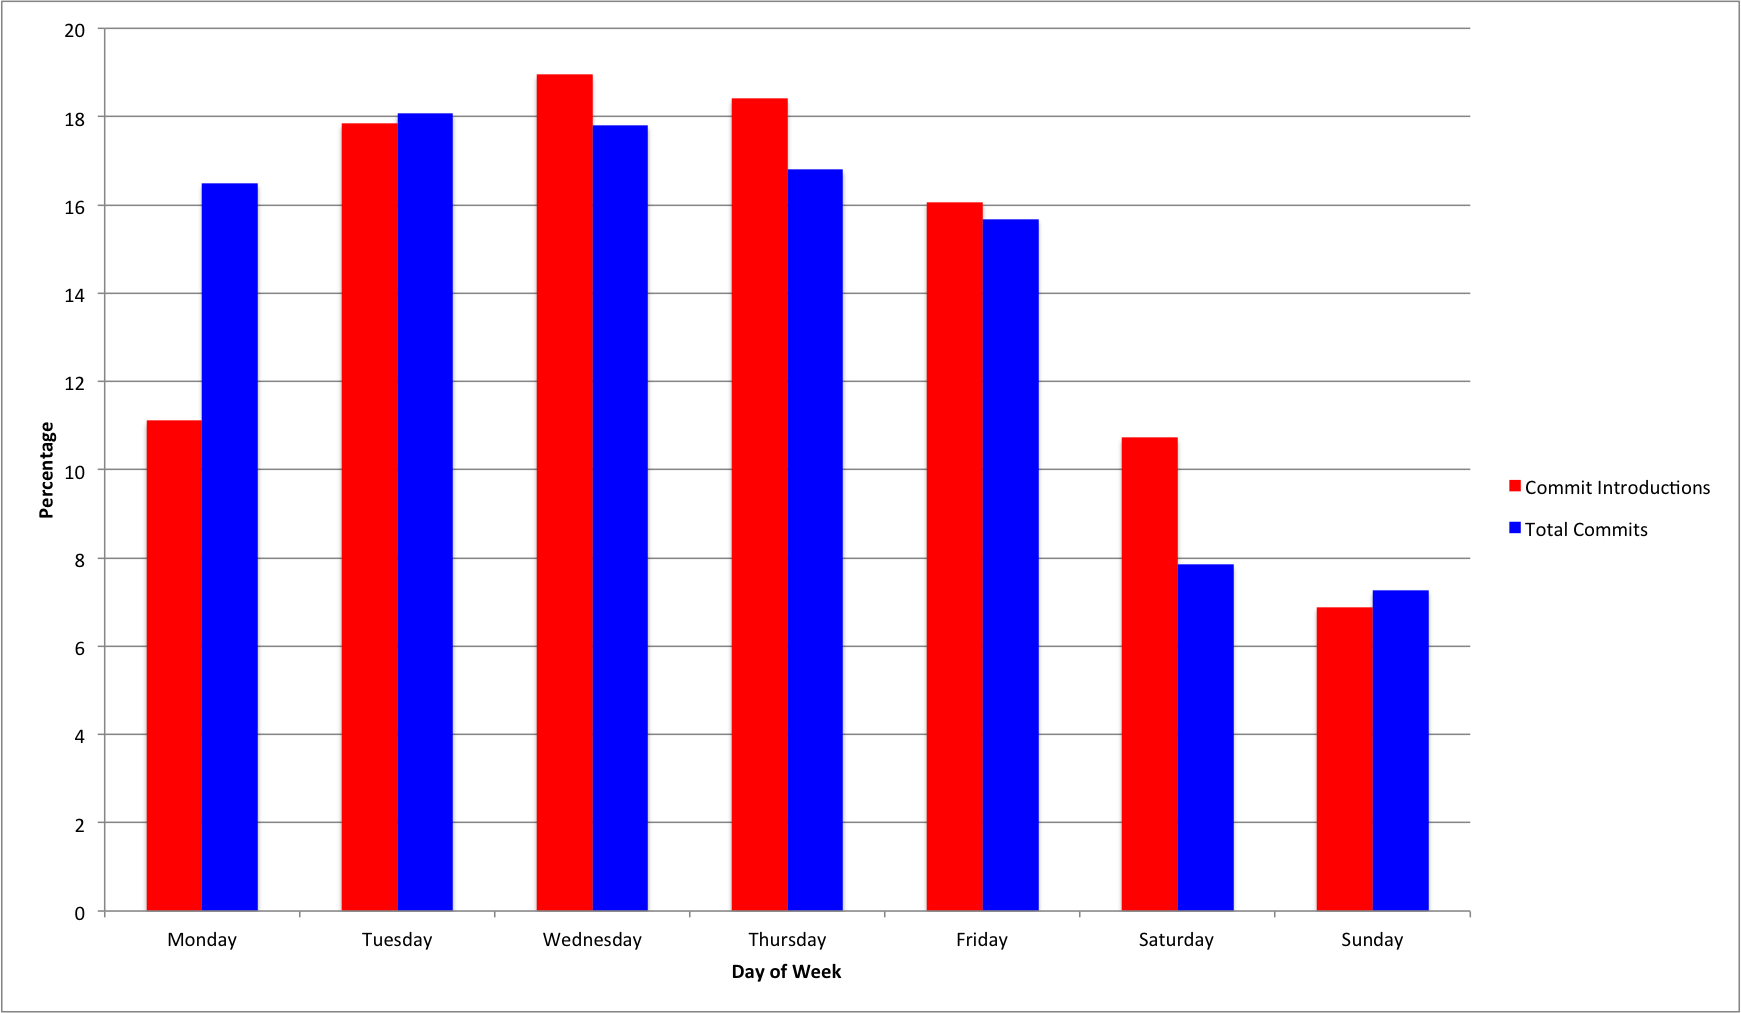
\includegraphics[width=0.9\textwidth]{linux_bug_introduction_day_of_week.png}
\end{center}
\caption{Linux percentage of bug introductions and percentage of total commits per day}
\label{fig-linux-weekday}
\end{figure*}

\begin{figure*}
\begin{center}
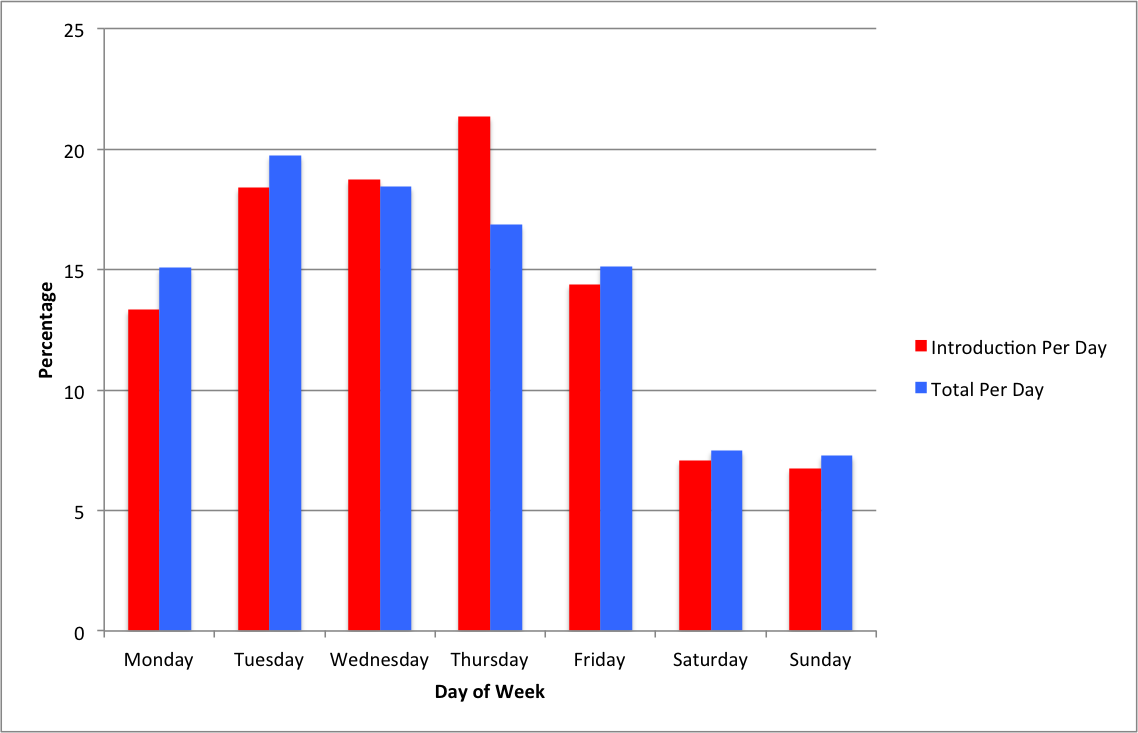
\includegraphics[width=0.6\textwidth]{firefox_bug_introduction_day_of_week.png}
\end{center}
\caption{Firefox percentage of bug introductions and percentage of total commits per day}
\label{fig-firefox-weekday}
\end{figure*}

First we determine if the day of the week has any impact on the
likelihood of producing bugs. For the following graphs the percentage
of introduction commits indicates the amount of commits out of the
total number of commits which are bug introductions. Our results from
Linux are shown in Figure \ref{fig-linux-weekday}. We see that
Saturday is the worst day followed by Thursday, while Monday has the
fewest percentage of bug introductions. The results for Firefox are
shown in Figure \ref{fig-firefox-weekday} and agree with Thursday
being one of the worse days while Monday is the best for committing
changes which do not introduce bugs. A possible explanation is that
developers rest over the weekend and have ample time to think about
the problem before writing it on Monday when they know exactly what to
do. It may also be correlated to the size of the change which we plan
to investigate later as an addition to our technique.

\begin{figure*}
\begin{center}
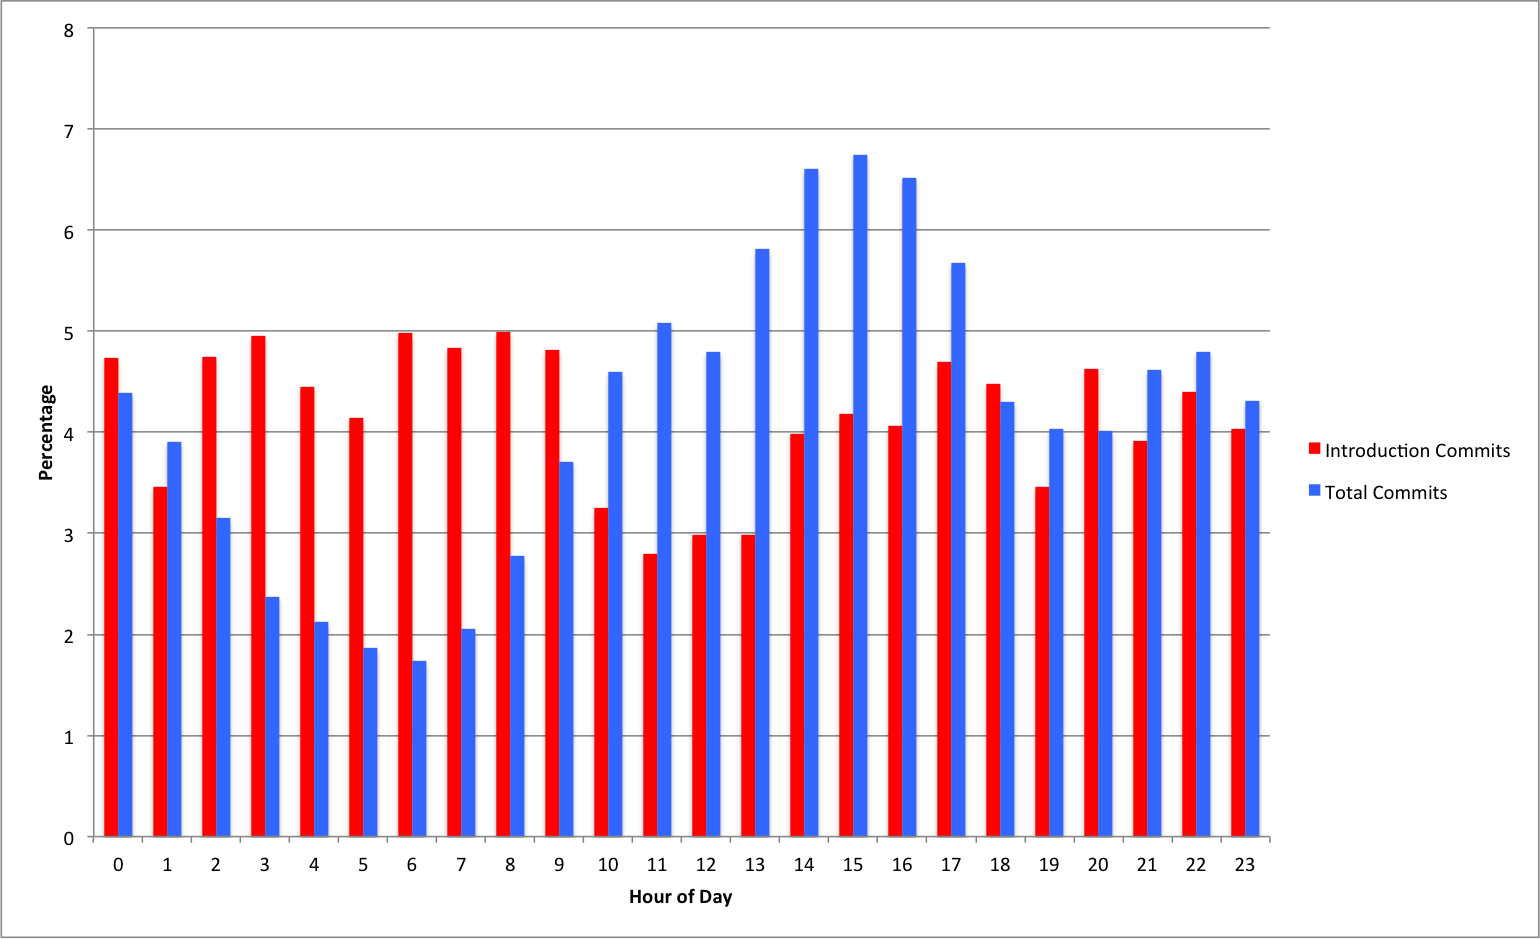
\includegraphics[width=0.9\textwidth]{linux_hour_of_day.png}
\end{center}
\caption{Linux percentage of bug introductions and percentage of total commits per hour}
\label{fig-linux-hour}
\end{figure*}

\begin{figure*}
\begin{center}
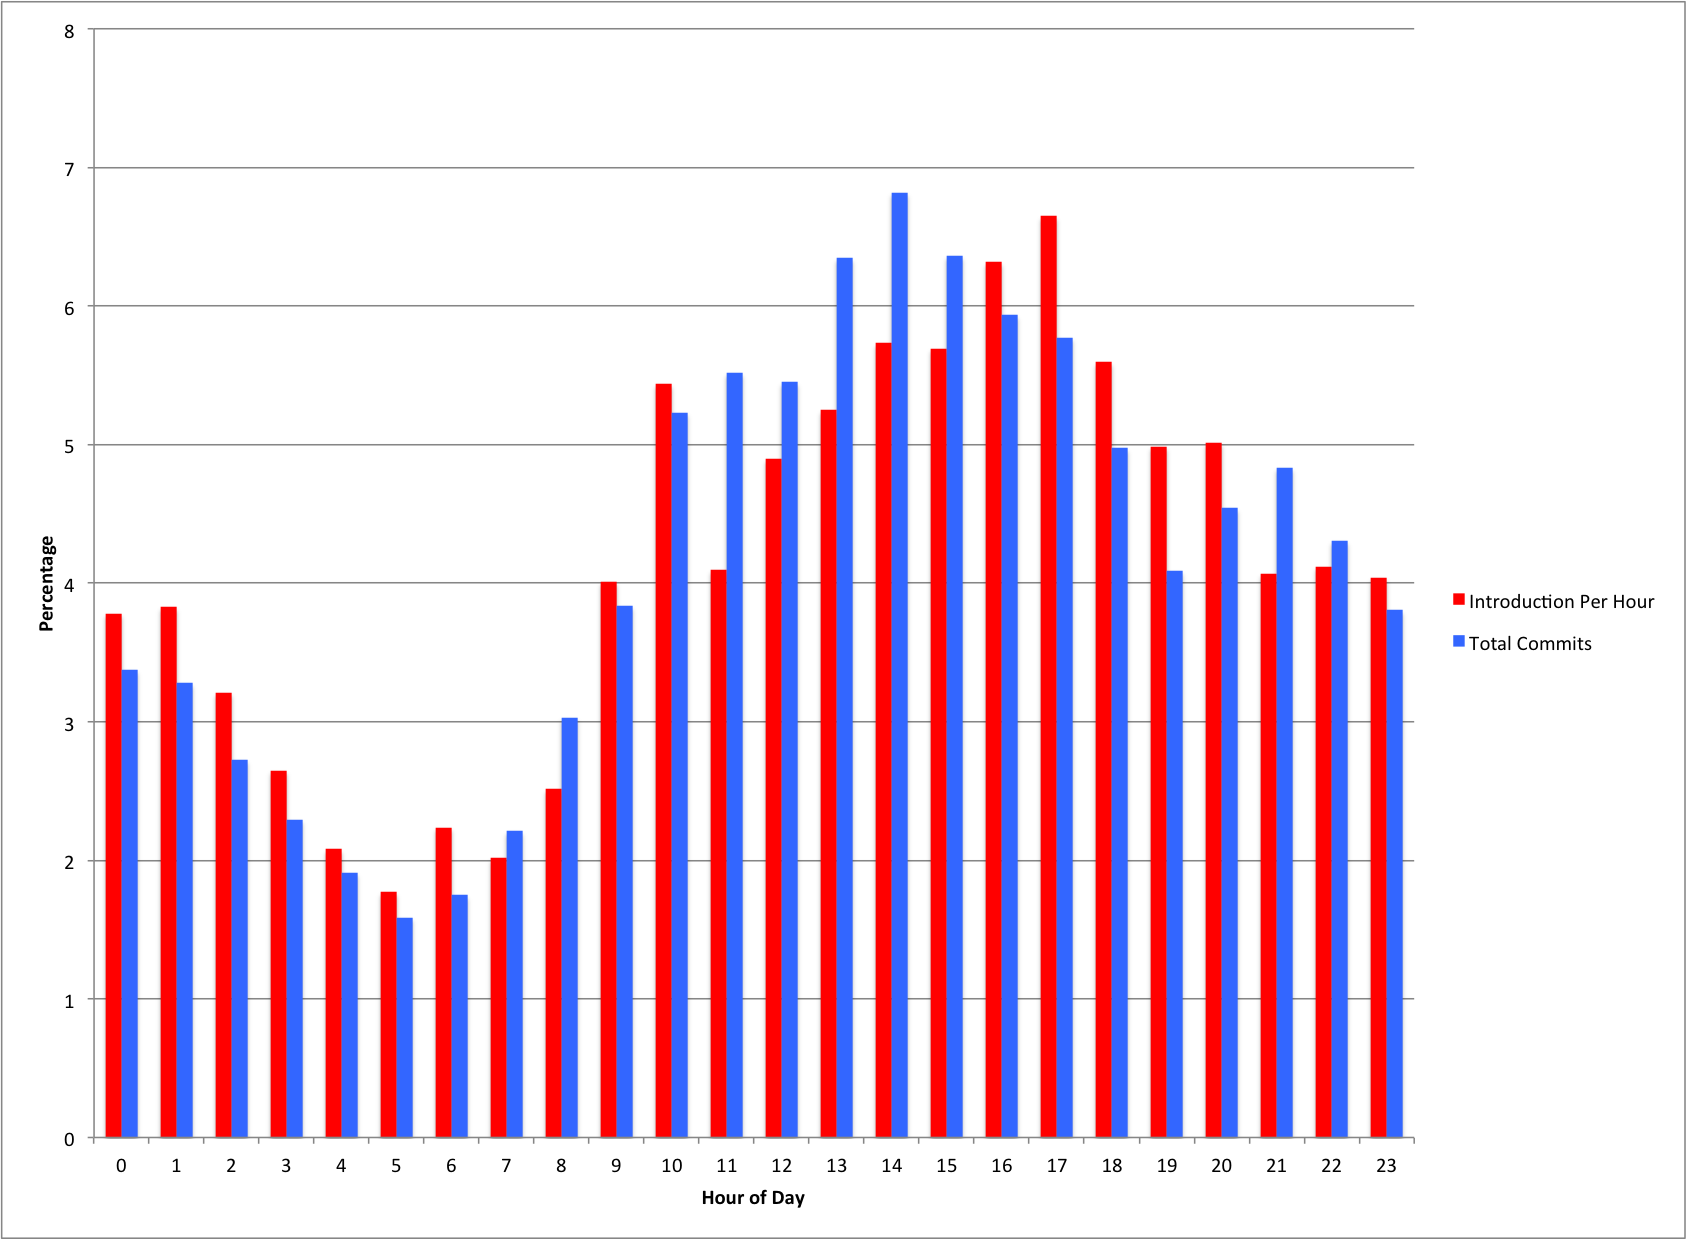
\includegraphics[width=0.9\textwidth]{firefox_hour_of_day.png}
\end{center}
\caption{Firefox percentage of bug introductions and percentage of total commits per hour}
\label{fig-firefox-hour}
\end{figure*}

Next we determine if the hour has any impact. Our results from Linux
and Firefox are shown in Figure \ref{fig-linux-hour} and Figure
\ref{fig-firefox-hour} respectfully. Both show a significant increase
in the amount of commits which introduce a bug between midnight and 9
AM. After this time there is a significant reduction in the amount of
bug introductions between 11 AM and 3 PM. After 3 PM however, the
likelihood of bug introductions fluctuates from hour to hour. This
result is not very surprising since tired programmers are more likely to
produce mistakes. It does however indicate the hours that programmers
are at the peak of their productiveness in terms of not creating
additional bugs.

\begin{figure*}
\begin{center}
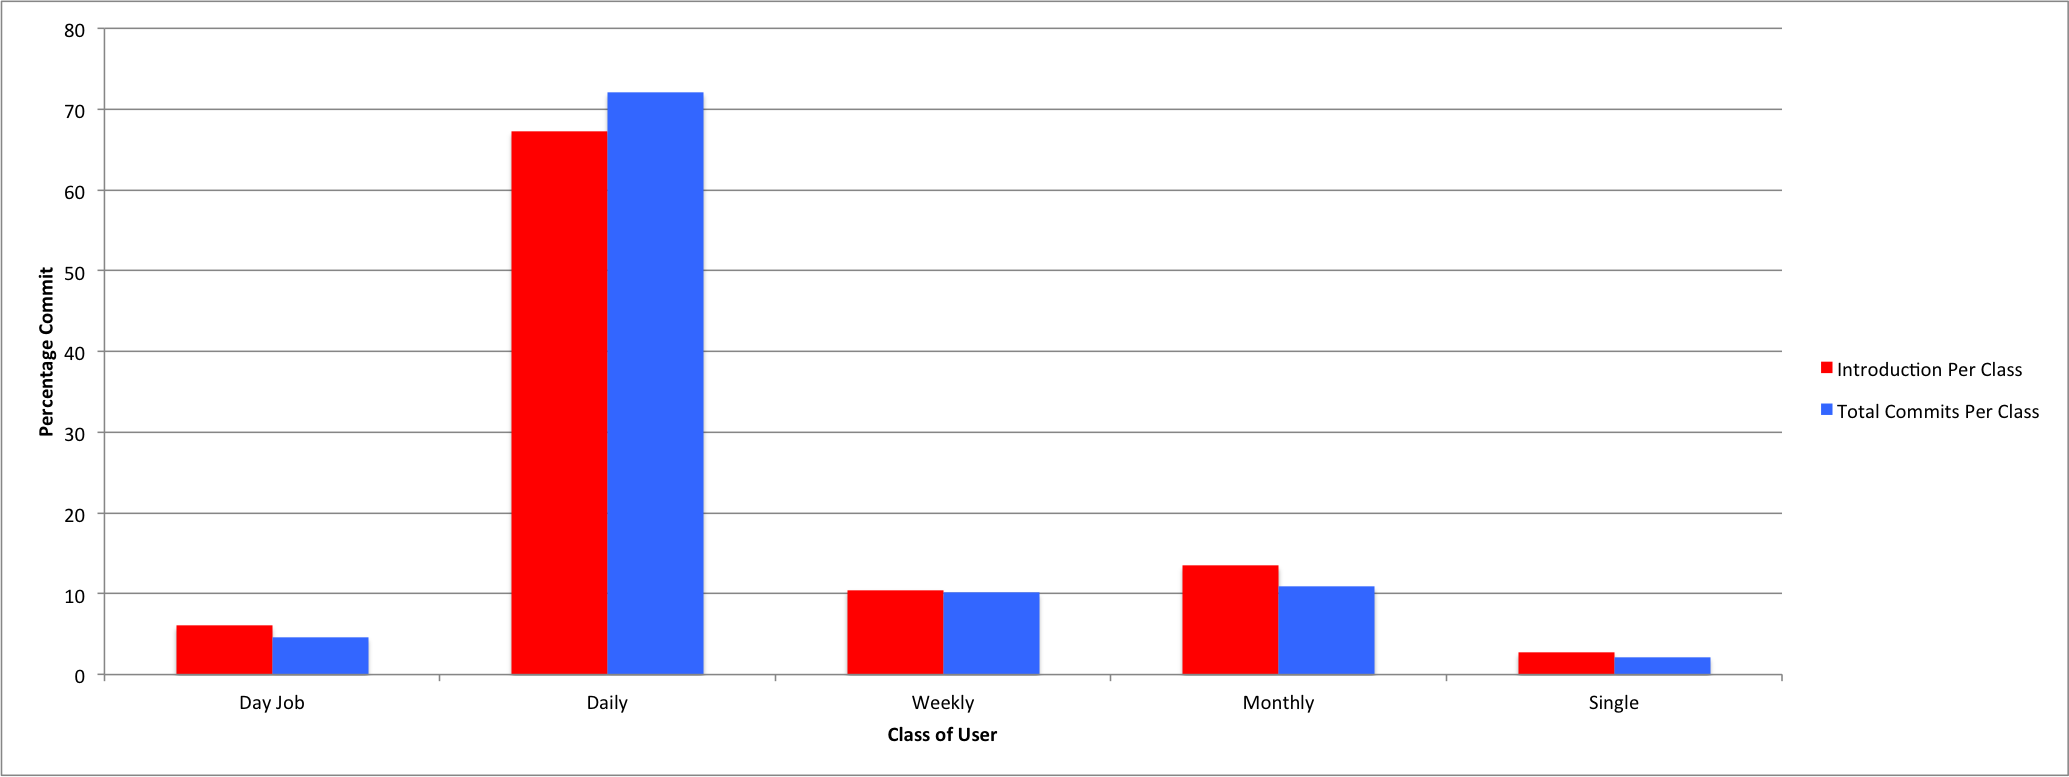
\includegraphics[width=0.9\textwidth]{linux_per_class.png}
\end{center}
\caption{Linux percentage of bug introductions and percentage of total commits per author classification}
\label{fig-linux-class}
\end{figure*}

\begin{figure*}
\begin{center}
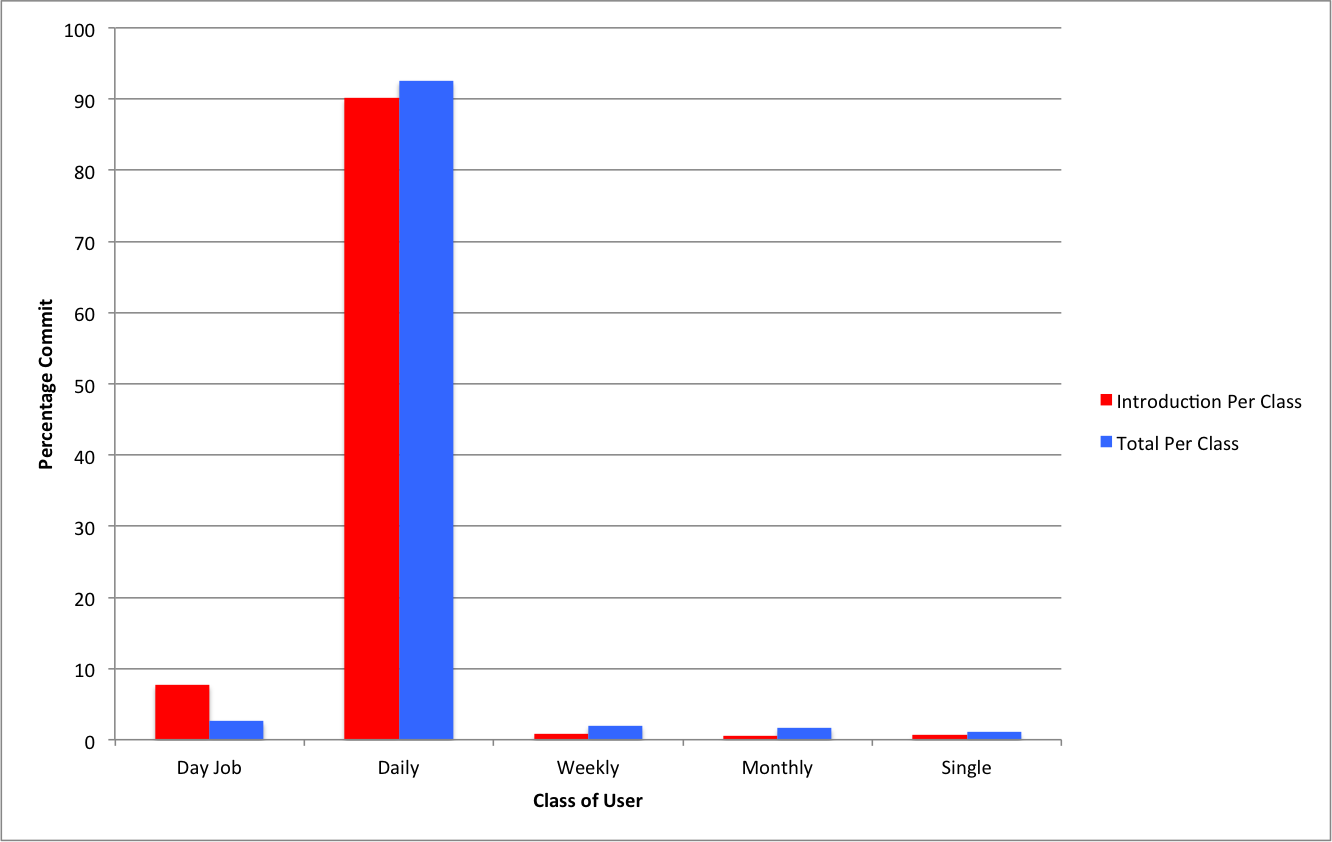
\includegraphics[width=0.6\textwidth]{firefox_per_class.png}
\end{center}
\caption{Firefox percentage of bug introductions and percentage of total commits per author classification}
\label{fig-firefox-class}
\end{figure*}

We then investigated how each classification of developers fair in
terms of their likelihood of creating a bug. The results from Linux
and Firefox are shown in Figure \ref{fig-linux-class} and Figure
\ref{fig-firefox-class} respectfully. We see that developers who
commit changes daily are a very significant portion of both projects
and not developers that work on code as part of their day job. This
trend is likely to be common to most open source projects. We also see
for both projects the daily developers are less likely to produce
bugs. On the other hand developers with this as their day job are more
likely to produce bugs. The cause of this could be that the developers
with this as their day job are required to make changes, while the
daily developers are motivated purely by interest.

\begin{figure*}
\begin{center}
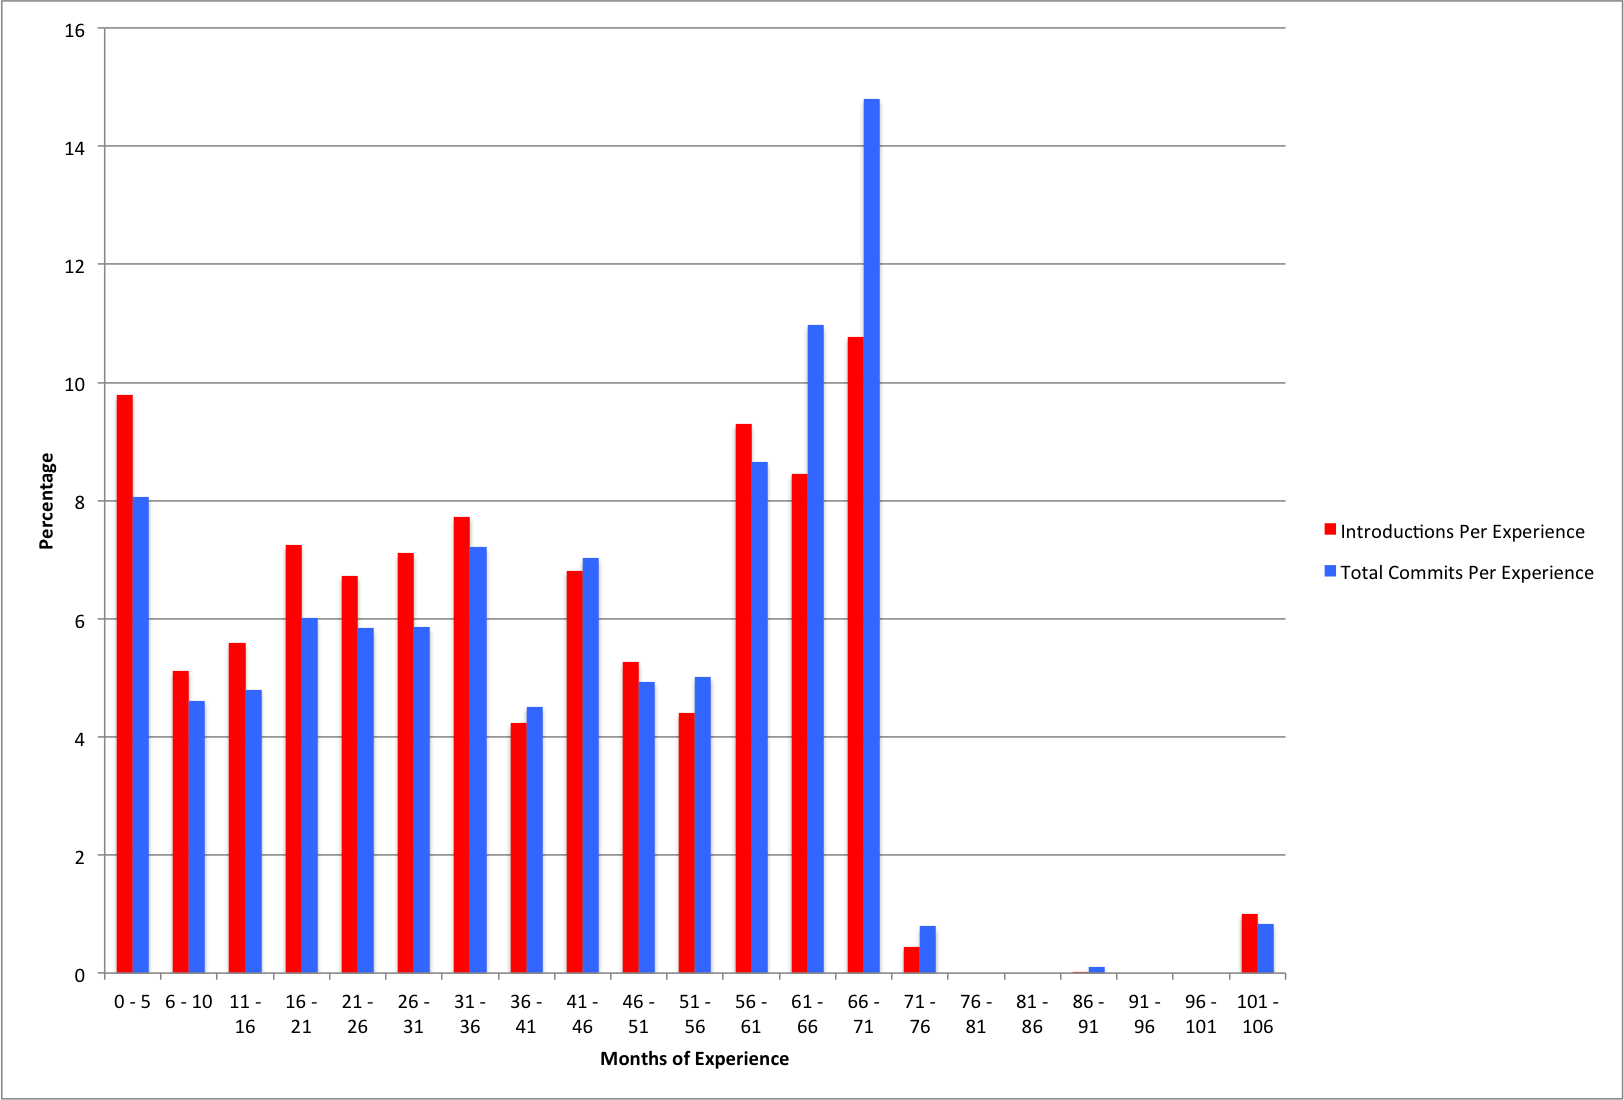
\includegraphics[width=0.9\textwidth]{linux_day_per_experience.png}
\end{center}
\caption{Linux percentage of bug introductions and percentage of total commits per author experience}
\label{fig-linux-experience}
\end{figure*}

\begin{figure*}
\begin{center}
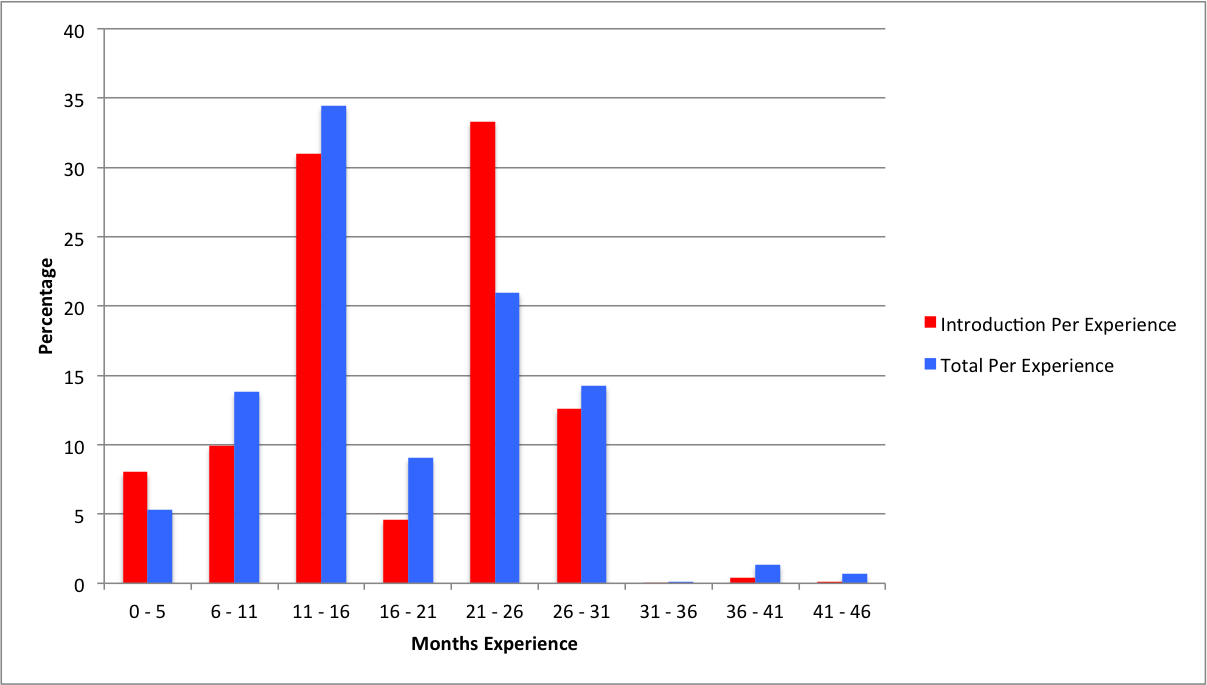
\includegraphics[width=0.6\textwidth]{firefox_day_per_experience.png}
\end{center}
\caption{Firefox percentage of bug introductions and percentage of total commits per author experience}
\label{fig-firefox-experience}
\end{figure*}

The final head-to-head comparison we performed is based on the amount
of experience per author. We divided them up into 6 months intervals. 
Our results from Linux and Firefox are shown in Figure
\ref{fig-linux-experience} and Figure \ref{fig-firefox-experience}
respectfully. For Linux authors with less than 2 years of experience
are more likely to commit a bug while after 2 years the likelihood
decreases. However the authors which committed throughout the history
of the project are more likely to commit a bug which may be because
they wrote the majority of the code. For Firefox, again the
developers with less than 6 months of experience are more likely to
commit a bug. The is a spike between 21 and 26 months as well. We
believe these results may not be accurate due to the possiblity of
our experience metric being crude and not representative of the 
actual experience with the project.

\begin{figure*}
\begin{center}
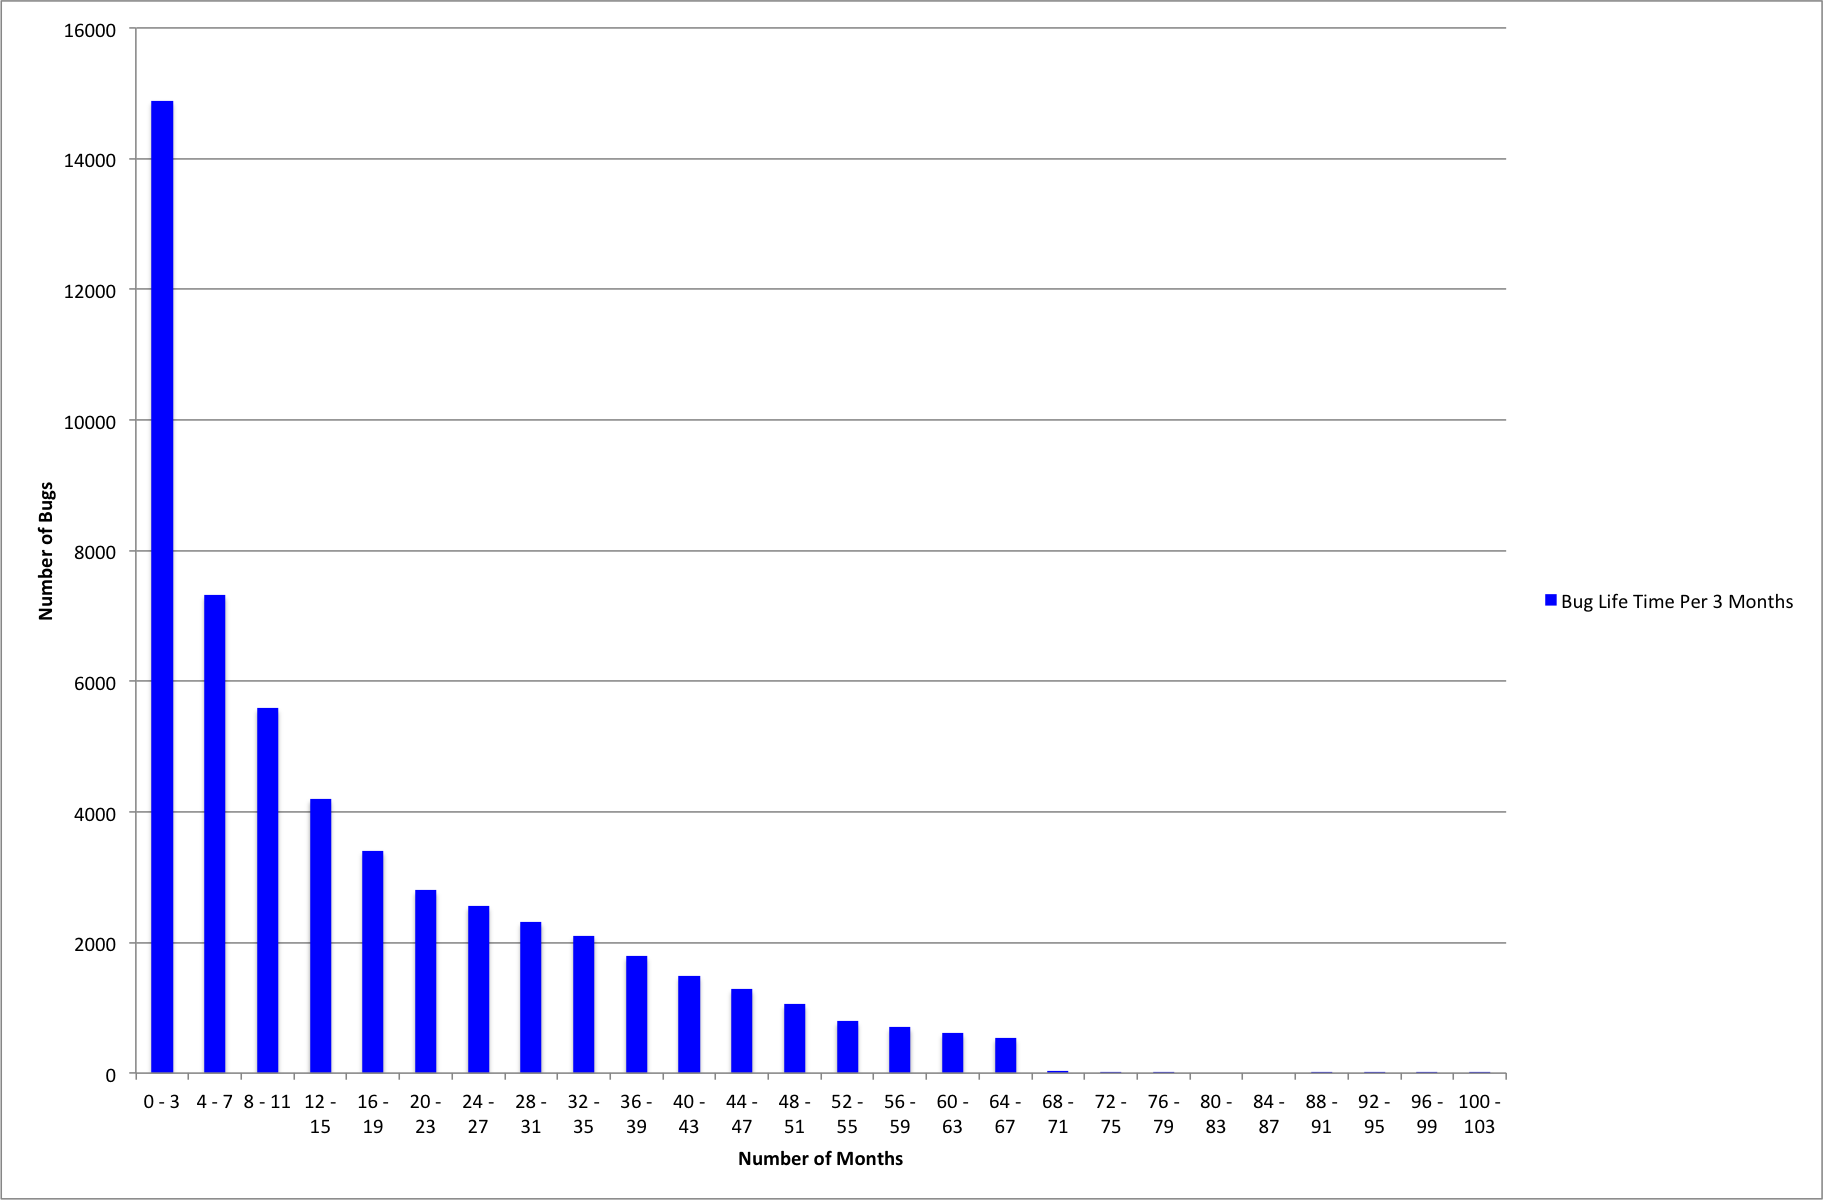
\includegraphics[width=0.9\textwidth]{linux_bug_life.png}
\end{center}
\caption{Linux number of bugs against bug lifetimes in months}
\label{fig-linux-buglife}
\end{figure*}

\begin{figure*}
\begin{center}
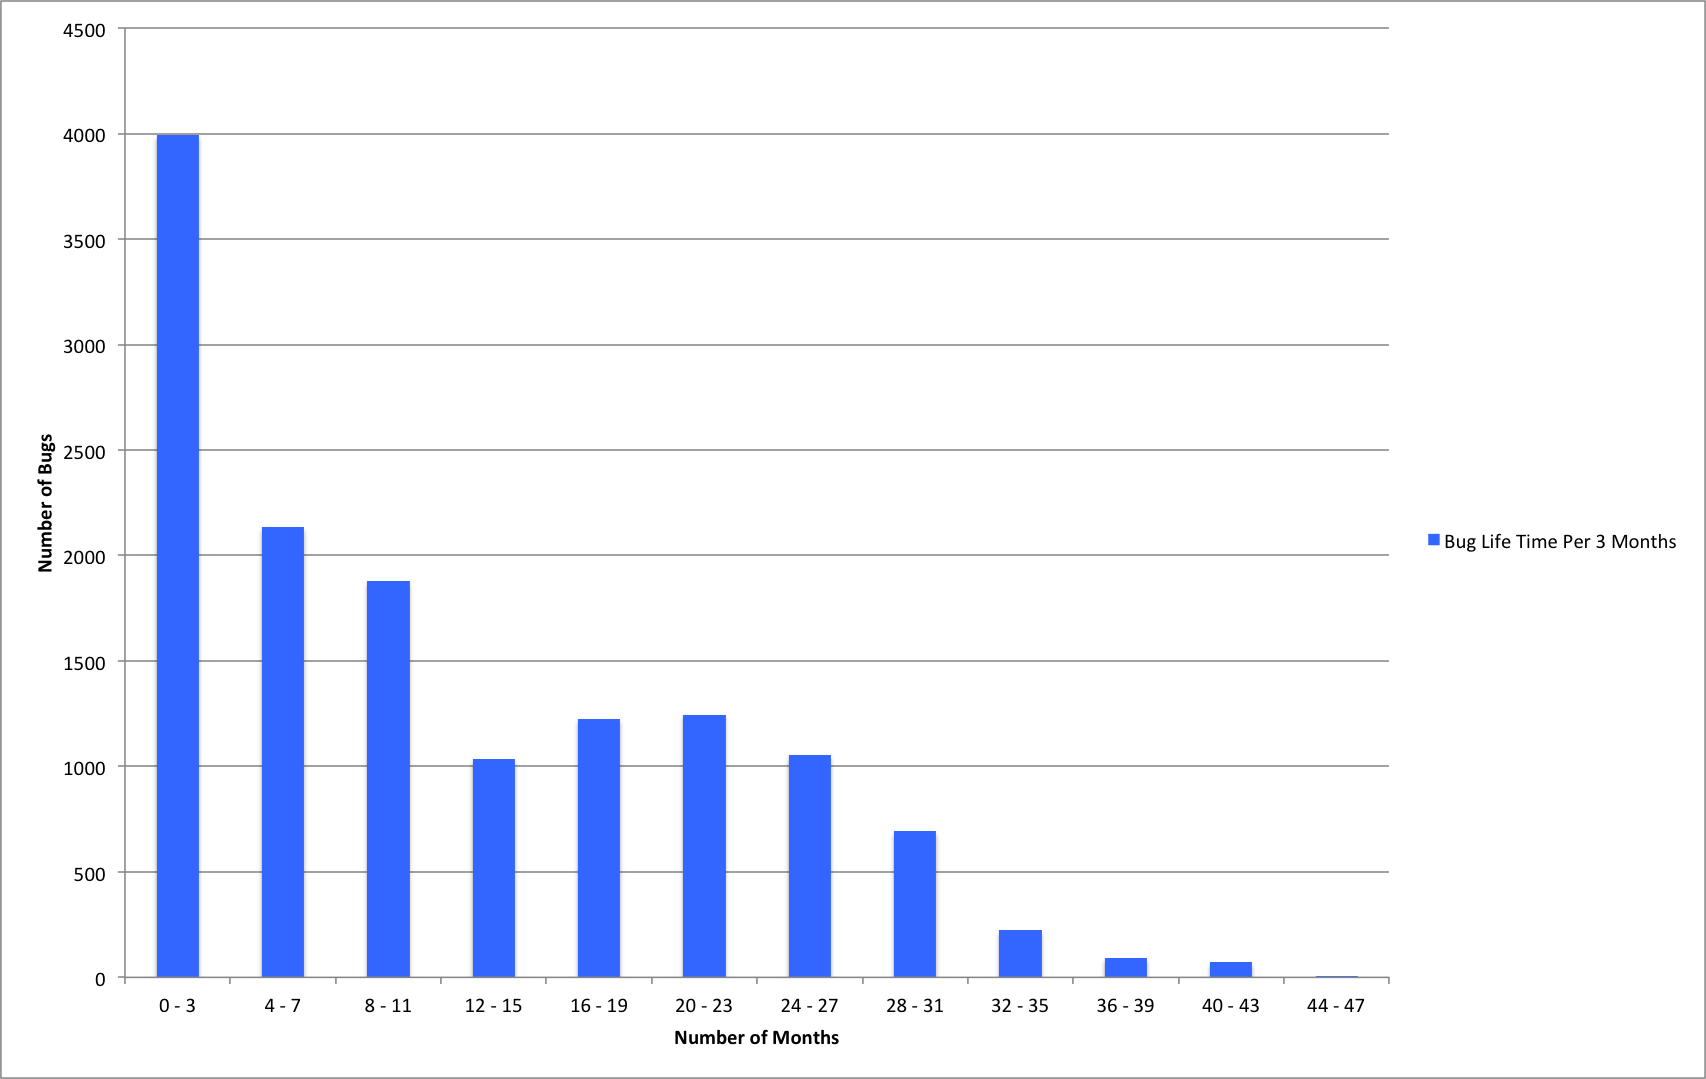
\includegraphics[width=0.9\textwidth]{firefox_bug_life.png}
\end{center}
\caption{Firefox number of bugs against bug lifetimes in months}
\label{fig-firefox-buglife}
\end{figure*}

Finally we determined the bug lifetimes for both projects to contrast
them to previous work. We plotted the number of bugs for each lifetime
divided into 4 month intervals. The results for Linux are shown in
Figure \ref{fig-linux-buglife}, the average bug lifetime is 1.39
years. The results for Firefox are shown in Figure
\ref{fig-firefox-buglife}, with an average bug lifetime of 0.97
years. This shows a reduction in the average bug lifetime for Linux (in
2002 the average lifetime was 1.8 years). This indicates that
developers are improving as their development process becomes more
refined. We also see the average lifetime is lower for Firefox, this
may be due to the complexity of the software, size of the software or
the amount of users (the more users and complex, the more likely bugs will be
revealed).

\section{Related Work}
\label{sec-related}

No single solution has been found for solving the problem of bug
introduction, but a lot of work has been done to try and minimize the
problem, because it is un-likely that it could be completely
resolved. Some of the things that could have been done is spend more
time on software design to minimize the introduction of design related
bugs by taking into account all the accumulated experiences to avoid
repeating any mistakes that lead to bugs. Finally, companies have made
strides in improving testing methodologies and automating the testing
process as much as possible, which lead to savings of approximately
\$22.5 billion \cite{2004-industry}. The works presented below are
mostly geared towards data collection for analysis, and trying to find
potential sources that could be contributing to bug-introducing
changes to see what can be done to minimize bug-introduction.

\paragraph{When do changed induce fixes?}
One of the relevant academic works is this paper, which analyzes CVS
achieves for fix-inducing changes. In other words, they examine code
changes that lead to problems. They discuss a methodology to
automatically locate fix-inducing changes by linking a version archive
to a bug database such as BUGZILLA \cite{2005-changes}. The authors
examined the history for Mozilla and Eclipse for their data
collection. The results they collected yielded that fix-inducing
changes show distinct patterns with respect to their size and the day
of the week they occurred. They discuss the general idea behind the
process of finding fix-inducing changes as: 1. Start with a bug report
in the bug database, indicating a fixed problem, extract the
associated change from the version archive to get the location of the
fix, and finally determine the earlier change at this location that
was applied before the bug was reported. The authors describe
syntactic and semantic analysis for the first step in the their
process of identifying potential fixes. Finally, through the use of
diff and annotate commands, as well as cycling through different
versions of the code, the authors are able to locate fix-inducing
changes. The study concluded that most bugs are introduced on Fridays
and Sundays. This work was important because it provided us with a
guideline for a methodology for extracting fix-inducing changes.

\paragraph{Automatic identification of bug-introducing changes}
The authors try to automate the process of finding bug-introducing
changes, which would remove the manual work associated with going
through bug reports or commit logs to collect this type of
information. They use the SZZ algorithm, which traces from the
location of the fix where the bug was introduced, and as such extract
the time \cite{2006-automatic}.The weakness with this algorithm is
that sometimes it makes false detections because not all modifications
are fixes, and a moderate improvement from using just SZZ is the use
of annotation graphs. Another improvement was ignoring format changes,
which reduce a large number of false positives. This paper has
inspired the approach we used for automating the process of
identifying bug-introducing changes, which was key for collecting a
large pool of data.

\paragraph{How long did it take to fix bugs?}
In this paper the author try to measure software quality as a function
of the number of bugs. The authors examine the bug fix time of files
in two open source software: ArgoUML and PostgreSQL, and tackle this
issue by identifying when bugs are introduced and when the bugs are
fixed \cite{2006-long}. The argument is files with the greatest
bug-fix times, whose bug counts are greater than average, may need
more attention to determine why bug fixes take such a long time –
potentially indicating the need for code refactoring to achieve faster
bug fixes in the future. The authors first extracted change histories
of the two projects, ArgoUML and PostgreSQL, using the Kenyon
infrastructure. To identify a bug-fix, they searched for keywords such
as fixed or bugs and they also searched for references to bug
reports. They then applied the identified bug-introducing changes by
applying the fix-inducing change identification algorithms described
in the paper “When do changes induce fixes?” which I mentioned
earlier.  This work is of course relevant because it gives us a
methodology for extracting bug-fix times.

\paragraph{If your bug database could talk}
This is another relevant work, where the authors perform experiments
that demonstrate how to relate developer, code, and process to defects
in the code. This work tries to understand why some programs are more
failure-prone than others.  To answer this question, we have to know
which programs are more failure-prone than others – to search for
properties of the programs or its development process that commonly
correlate with defect density. The authors try to answer questions
like “can one predict failure-proneness from metrics like code
complexity?”, “what does a high number of bugs found after release?”,
and “do some developers write more failure-prone code than
others?”. After examining Eclipse database, some of the conclusions
that the authors made were: new or combination of existing metrics
need to be explored to study the relationship between complexity of
code to the presence of bugs in a given class, it is difficult to
predict post-release failures solely from process measurements, and
there is a high variance in failure density in files owned by
different developers \cite{2006-if}. Their methodology for extracting
information from bug reports from BUGZILLA will be very useful for our
project.

\paragraph{On the Nature of Commits}
This paper studies the nature of commits in two dimensions: define the
size of commits in terms of number of files, and classify commits
based on the content of their comments \cite{hattori2008nature}. The
authors investigated the distribution of commits according to the
number of files, and their results show that the majority of commits
contain a large number of files. The authors also developed a
classification system for commits according to development and
maintenance activities based on the content of their commits, a system
that is more suitable for open source projects. Some of the major
findings made by the authors include: the majority of the commits are
not related to the development activities, corrective actions generate
more tiny commits, and development activities are spread among all
sizes of commits.

\section{Future Work}
\label{sec-future}

There are a few parts of the implementation which could be improved to
reduce the number of false positives. First, our fix detection for
commit messages is very simplistic and could be improved to determine
fixes which do not refer to any bugs. We can also introduce additional
logic to ignore code which has been moved or renamed. The author
information for experience also did not seem reliable, due to the fact
that we treat every name and e-mail pair as a unique author. However, this
might not be the case if the authors simply changed their e-mail address. 

We could also add additional extensions to the database including: categorizing
authors by their official roles, and classifing the size of each commit as
well to determine if larger commits are more likely to contain bugs.

In addition we would like to add additional software projects to the
database. Another goal is to release the data to the community so
others may extend and add to it. We believe there are much more
interesting results which could be found using our database.

\section{Conclusion}
\label{sec-conclusion}

Resolving bugs represent a substantial amount of time and cost in
software projects. It is important to investigate the cause of bugs in
order to reduce the amount of bugs which occur. We believe that the
data we have collected will be beneficial for the software quality
assurance and software developing personnel to use the correlations we
found, and investigate other possible correlations from the data we
collected and stored in a database. From manually checking a random
sample we found our data to be representative. Our data has
revealed that Thursdays have a high bug introduction rate relative to
the total number of commits for that day, while Mondays have the
lowest bug introduction rates. There may be many reasons behind this
correlation, but we believe it might be that people are being worn out towards the
end of the week, and as such are more likely to introduce bugs, except
this would mean that Fridays would be worst - which is not the
case. It could also be that on Fridays people are more alert and focused
because they are excited for the weekend. It was strange that Mondays
yielded the best results for time to code, but this could be the case
because people are just back from the weekend and they are fully
charged, ready to work. Another possible theory for Monday's results,
which is that people delegate easier tasks for Mondays because its the
start of the week, or spend more time planning and laying out
templates of what they will be coding, and as such are not as prone to
introducing bugs. This of course could be proven by checking the size of
the commits and what kind of changes are being made on Mondays. Our
data also showed that coding between 12AM and 9AM is a bad idea, while
the best time is between 11AM and 3PM. This is not a very surprising
result, considering how most users sleep during these hours, and if
they happen to be doing any coding during these hours, it would be
considered to be outside of their usual working hours - making them
more prone to errors.  From our commits that were organized by author
classification, it seems that daily committers are less prone to bug
introduction than those who are classified as day job users. One
theory that could potentially explain this result is that hobbyist
working on open source projects do it because they are highly
interested, while day job users are doing it to get payed, so the
difference in motivations could negatively affect the performance
of the developer. Finally our data shows that bug lifetimes decay
exponentially, and on average are longer for larger projects. This
result of course is positive because it indicates that the majority of
bugs are dealt with fairly quickly.

%% \acks
%% Acknowledgments, if needed.

% We recommend abbrvnat bibliography style.
\bibliographystyle{abbrvnat}

% The bibliography should be embedded for final submission.
\nocite{*}
\bibliography{references}

%% \appendix
%% \section{Linux}

\end{document}
